\renewcommand{\thefigure}{A\arabic{figure}}
\setcounter{figure}{0}
\renewcommand{\thetable}{A.\arabic{table}}
\setcounter{table}{0}
\renewcommand{\thesection}{A.\arabic{section}}
\setcounter{section}{0}

\section*{Appendix}

\subsection*{Model Layout}

\begin{align*}
  Likelihood:& \\
  Y_{i} &\sim Continuation-Ratio(\mu_{i}, \tau_{k}) \\
  Linear Model:& \\
  \mu_{i} &= X_{i} \beta + W_{i}\eta_{k} + \alpha_{j}[i] \\
  Priors:& \\
  \beta_{p} &\sim T(0, 10, 3), \text{ for } p = 1, \ldots p \\
  \eta_{qk} &\sim T(0, 10, 3), \text{ for } q = 1, \ldots Q \text{ and } k =1, \ldots, K-1 \\
  \tau_{k} &\sim N(0, 1.5), \text{ for } k = 1, \ldots, K-1 \\
  \alpha_{j} &\sim N(0, \sigma_{\alpha}) \\
  Hyperpriors:& \\
  \sigma_{\alpha} &\sim Exponential(2)
\end{align*}

To describe our model we use the convention in \citet{mcelreath2016statistical}. The first two lines describe the likelihood and linear model and the remaining define the prior distribution for each parameter in the model. Let $Y_{i}$ be a particular country-year observation's score on our dependent variables. Both of our dependent variables take an integer value of $k=1, \ldots, K$. The framework we presented in our paper treats $Y_{i}$ as a function of a normally-distributed latent variable with a mean of $\mu$ and a standard deviation of 1. The $k=1, \ldots, K-1$ threshold parameters, $\tau$, partition this distribution into $K$ sections. The area of each of these sections describe the probability of falling into each response category.

To model changes in these probabilities, the models assume $\mu$ to be an additive combination of linear effects. We parameterize this model via first a set of variables, $X$ that are thought to effect the probability of falling into a particular category equally and the effect of these variables is captured by a $P$ length vector of coefficients, $\beta$. We also include $Q$ variables that have category specific effects and these are denoted by $W$ and their effect is measured by $\eta$. $\alpha$ represents a set of varying effects that account for country-ICC case specific unmeasured variation.

For both the \emph{State- and Opposition-Focused ICC Transition} models we utilize the same set of prior distributions. For $\beta$ and $\eta$ we use Student's t priors with three degrees of freedom. For the threshold parameters, $\tau$, we use a Normal distribution with a mean of zero and standard deviation of 1.5. We also use normally distributed priors for $\alpha$ and set the mean to zero and standard deviation to $\sigma_{\alpha}$, which  has its own Exponential hyperprior with a rate of 2.

\subsection*{Convergence Check for Main Models}

Below we show trace plots, after a burn-in period of 4,000 iterations, for both the \emph{State- and Opposition-Focused ICC Transition} dependent varibales. In both cases, we can see that the chains seem to be mixing well and have converged.

\begin{figure}
    \centering
    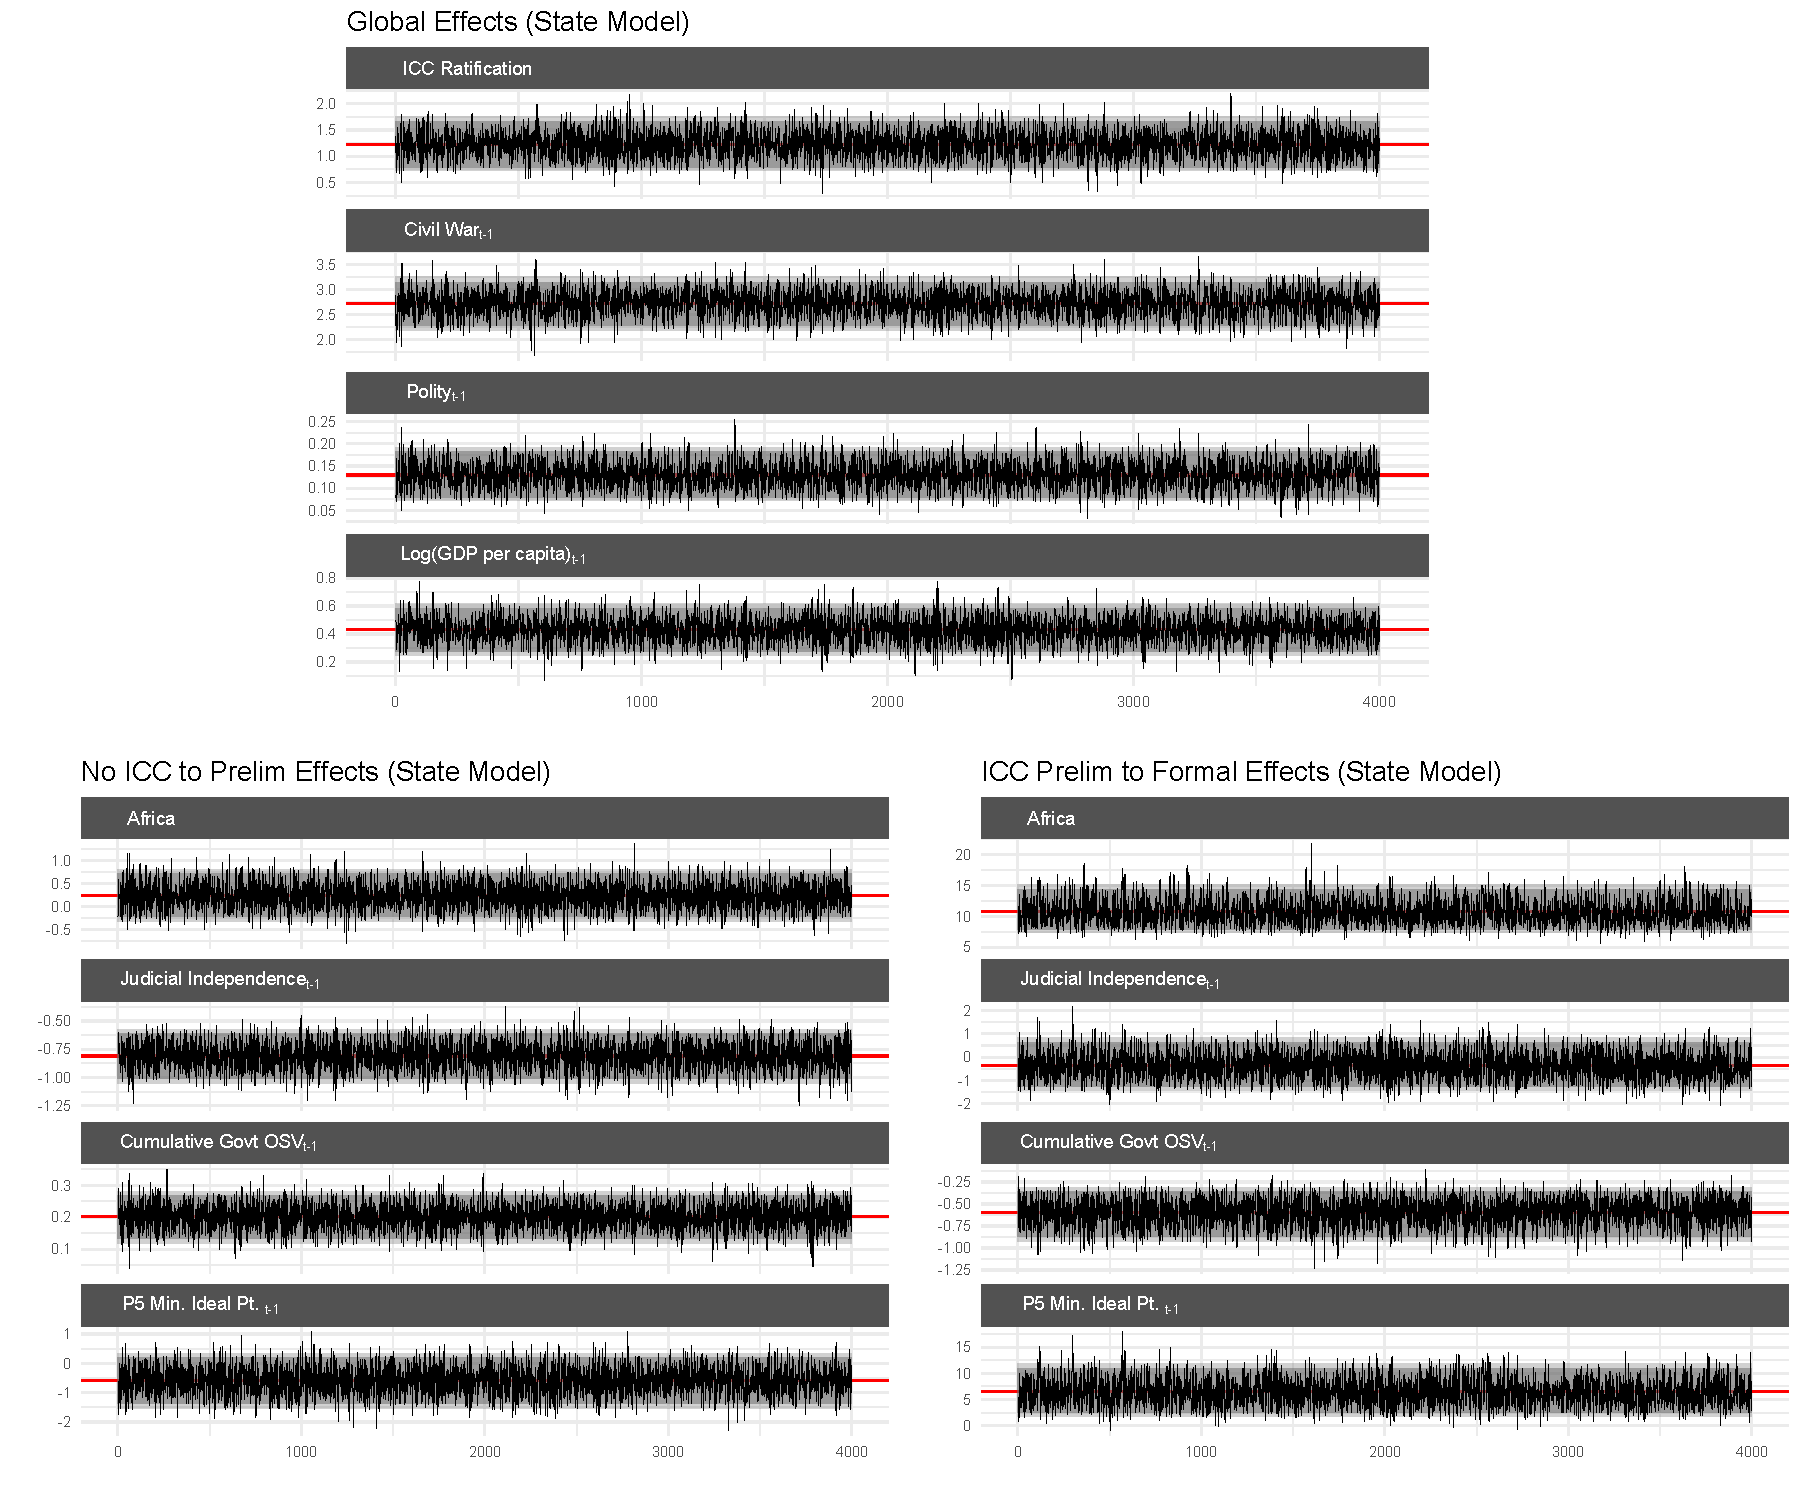
\includegraphics[width=1\textwidth]{stateCoefTrace.pdf}
    \caption{Trace plot for \emph{State-Focused ICC Transition} model.}
    \label{fig:stateTrace}
\end{figure}
\FloatBarrier

\begin{figure}
    \centering
    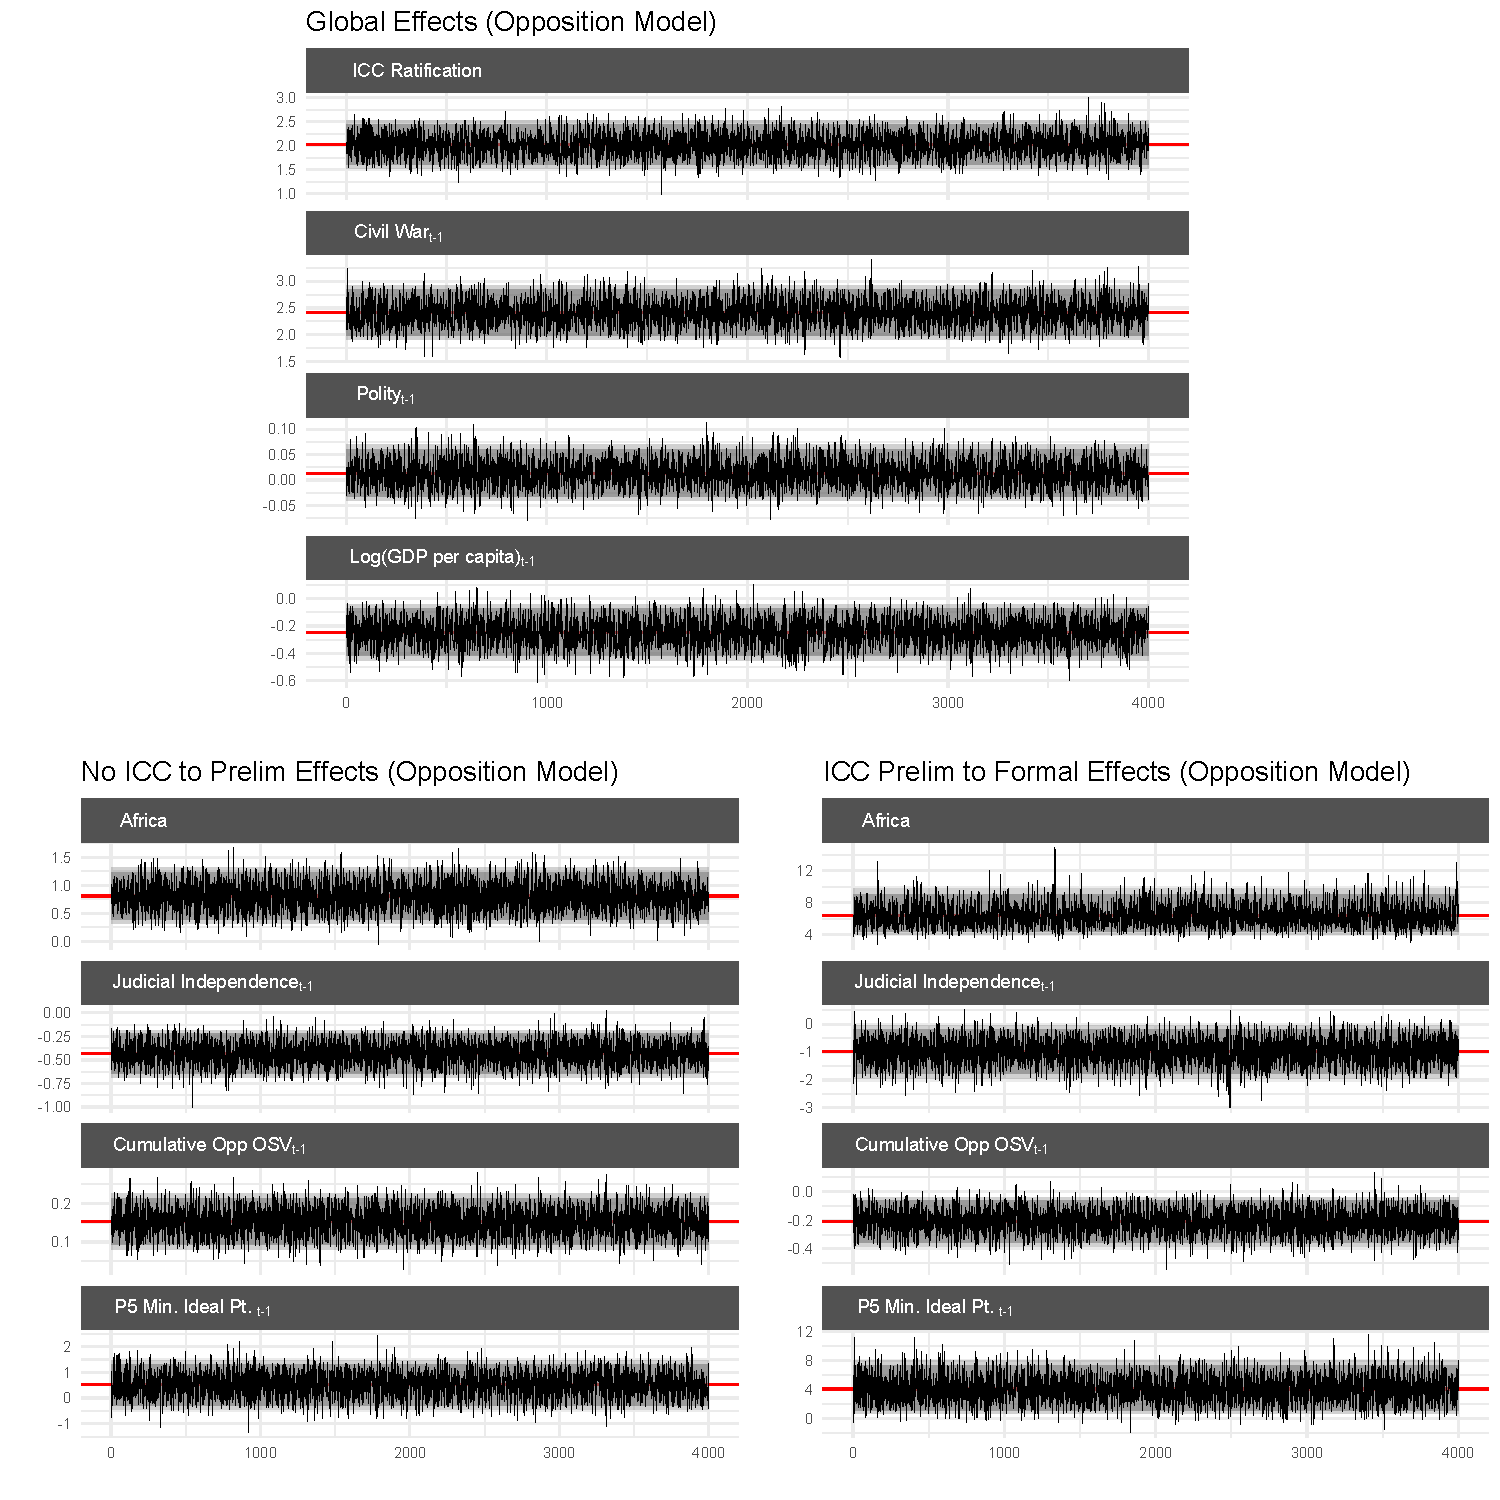
\includegraphics[width=1\textwidth]{rebelCoefTrace.pdf}
    \caption{Trace plot for \emph{Opposition-Focused ICC Transition} model.}
    \label{fig:oppTrace}
\end{figure}
\FloatBarrier

\subsection*{PTS \& ICC Ratifier Robustness Check}

% pts greather than 3 andd icc ratif equals 1

We examine the robustness of our results to a sample restriction. Specifically, we subset our sample to those cases where the PTS value is greater than three and only ICC ratifiers. Results are shown below and are broadly similar to what we report in the paper.

\begin{figure}
    \centering
    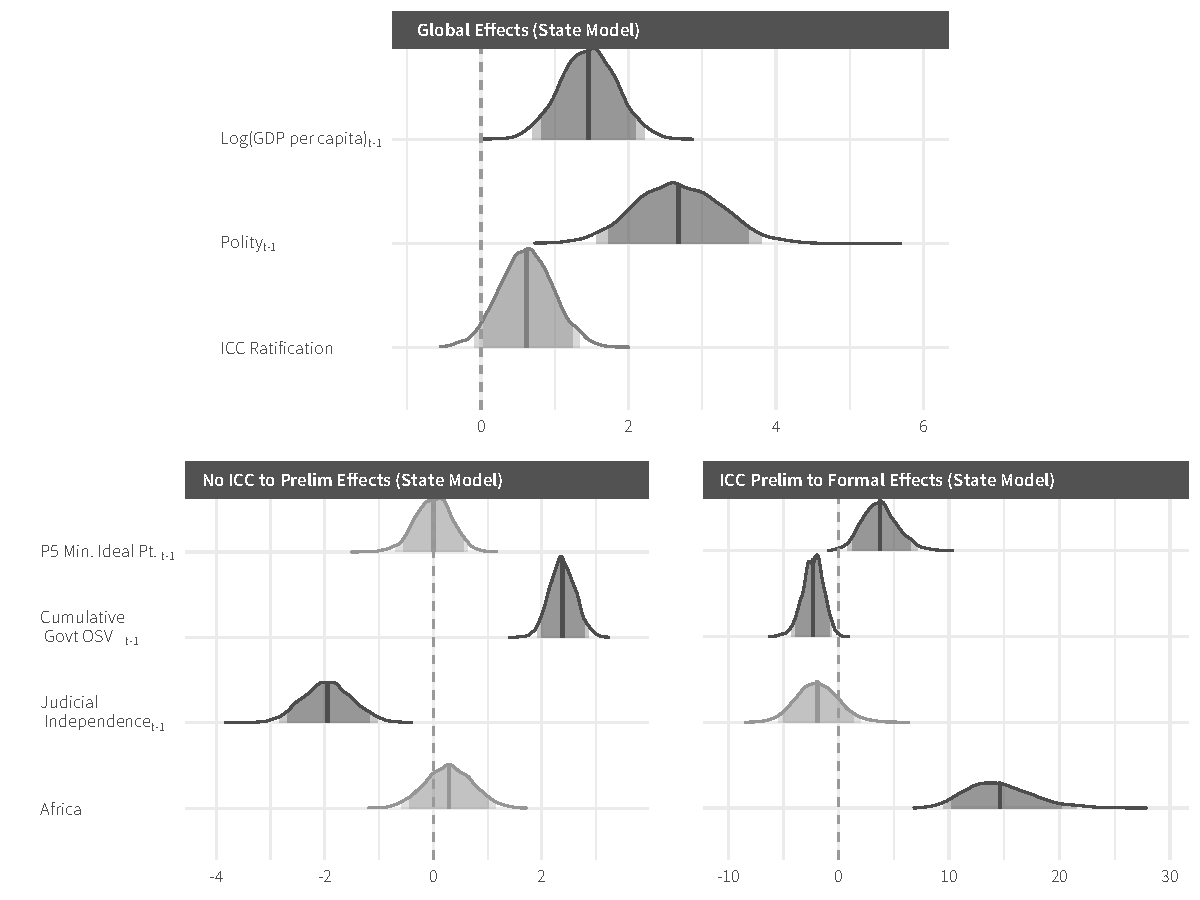
\includegraphics[width=1\textwidth]{stateCoefSumm_ptsCivilWarOnly.pdf}
    \caption{Parameter estimates when restricting sample to PTS greater than three and only ICC ratifiers from State-Focused ICC Transition model visualized through posterior distributions with median values designated by vertical line, lightly shaded portion indicating the 95\% credible interval, and darker shaded portion the 90\% credible interval.}
    \label{fig:stateModel_pts3_icc1}
\end{figure}

\begin{figure}
    \centering
    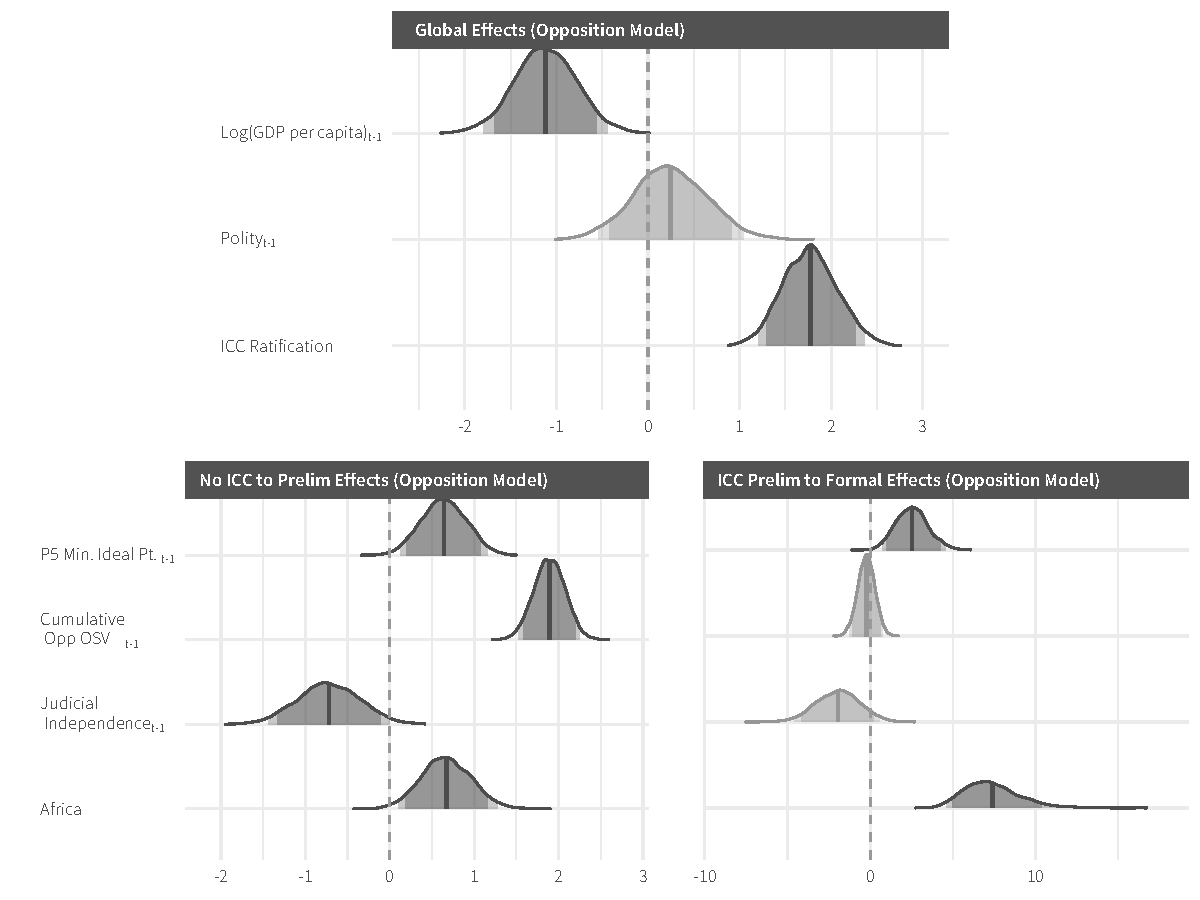
\includegraphics[width=1\textwidth]{rebelCoefSumm_ptsCivilWarOnly.pdf}
    \caption{Parameter estimates  when restricting sample to PTS greater than three and only ICC ratifiers from Opposition-Focused ICC Transition model visualized through posterior distributions with median values designated by vertical line, lightly shaded portion indicating the 95\% credible interval, and darker shaded portion the 90\% credible interval.}
    \label{fig:rebelModel_pts3_icc1}
\end{figure}

\subsection*{Results without imputation}

To make sure that our results are not being driven by our multiple imputation procedure we also run a version of our sampler in which we employ listwise deletion. The results are shown below and are broadly similar to those reported in the paper.

% Results broadly the same ... p5min ideal point in no icc to prelim eff same direction but no longer sig, africa in no icc to prelim same direction but no longer sig ... everything else the same

\begin{figure}
    \centering
    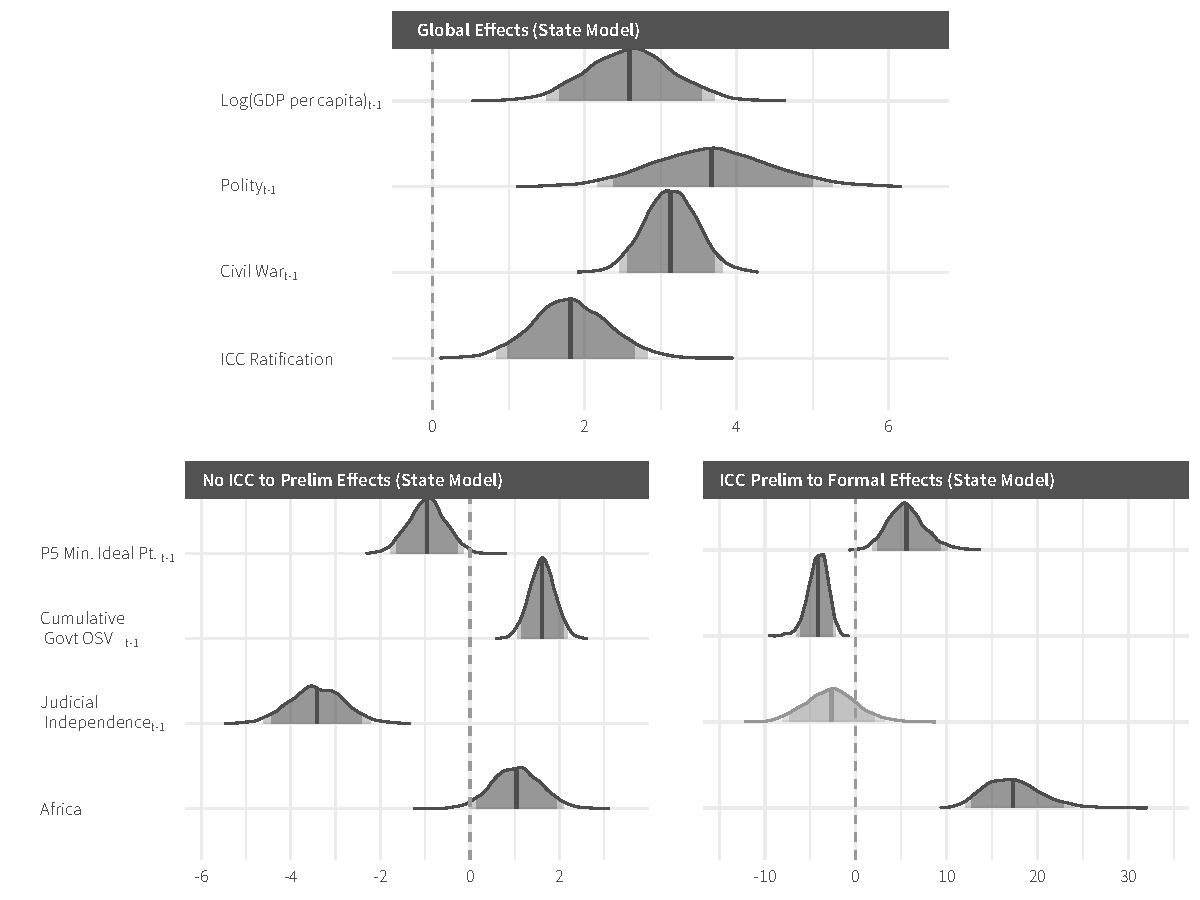
\includegraphics[width=1\textwidth]{stateCoefSumm_noImp.pdf}
    \caption{Parameter estimates when using listwise deletion from State-Focused ICC Transition model visualized through posterior distributions with median values designated by vertical line, lightly shaded portion indicating the 95\% credible interval, and darker shaded portion the 90\% credible interval.}
    \label{fig:stateModel_noImp}
\end{figure}

% Results broadly the same ... evidence stronger for cumm opp osv in icc prelim to formal effects

\begin{figure}
    \centering
    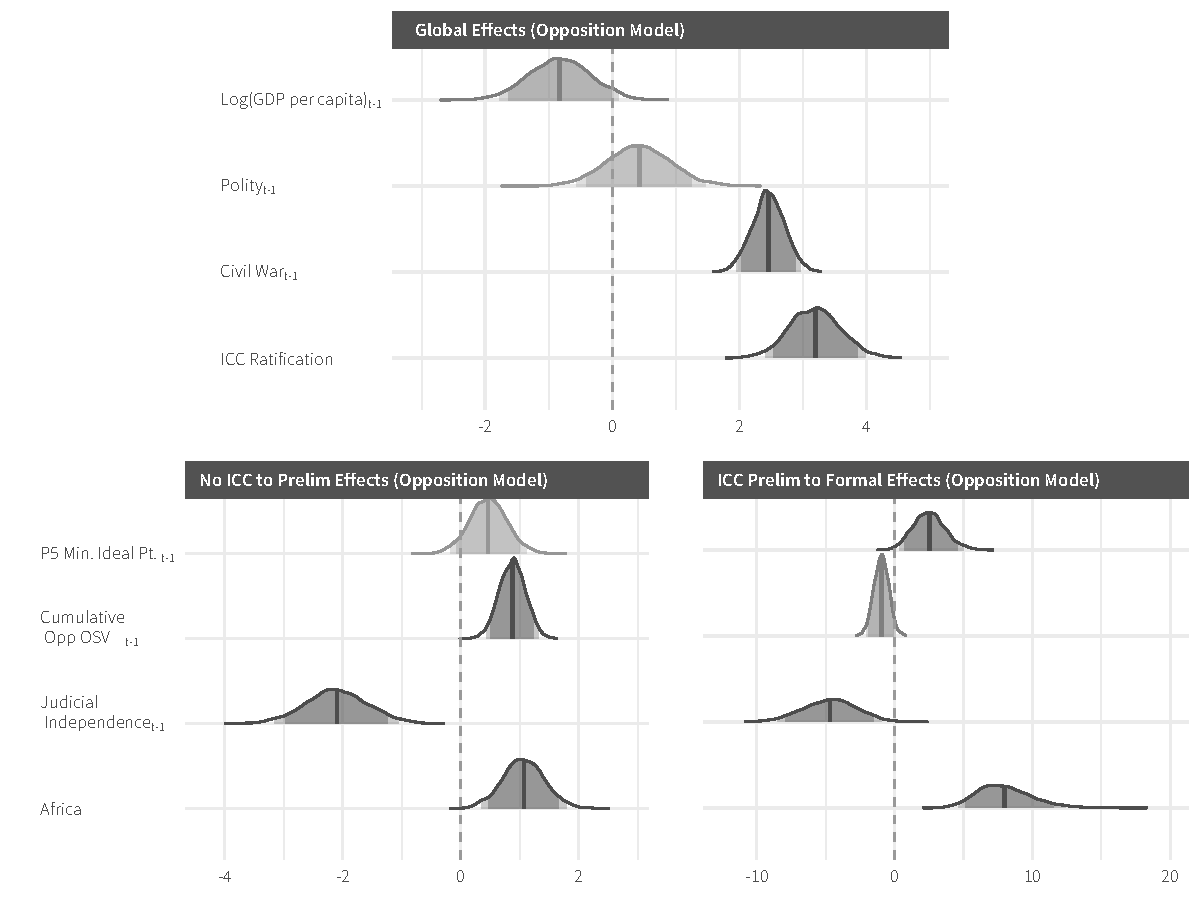
\includegraphics[width=1\textwidth]{rebelCoefSumm_noImp.pdf}
    \caption{Parameter estimates when using listwise deletion from Opposition-Focused ICC Transition model visualized through posterior distributions with median values designated by vertical line, lightly shaded portion indicating the 95\% credible interval, and darker shaded portion the 90\% credible interval.}
    \label{fig:rebelModel_noImp}
\end{figure}

\subsection*{Comparison with ordinal logit}

To show the utility of our approach we also compare it against

\begin{figure}
    \centering
    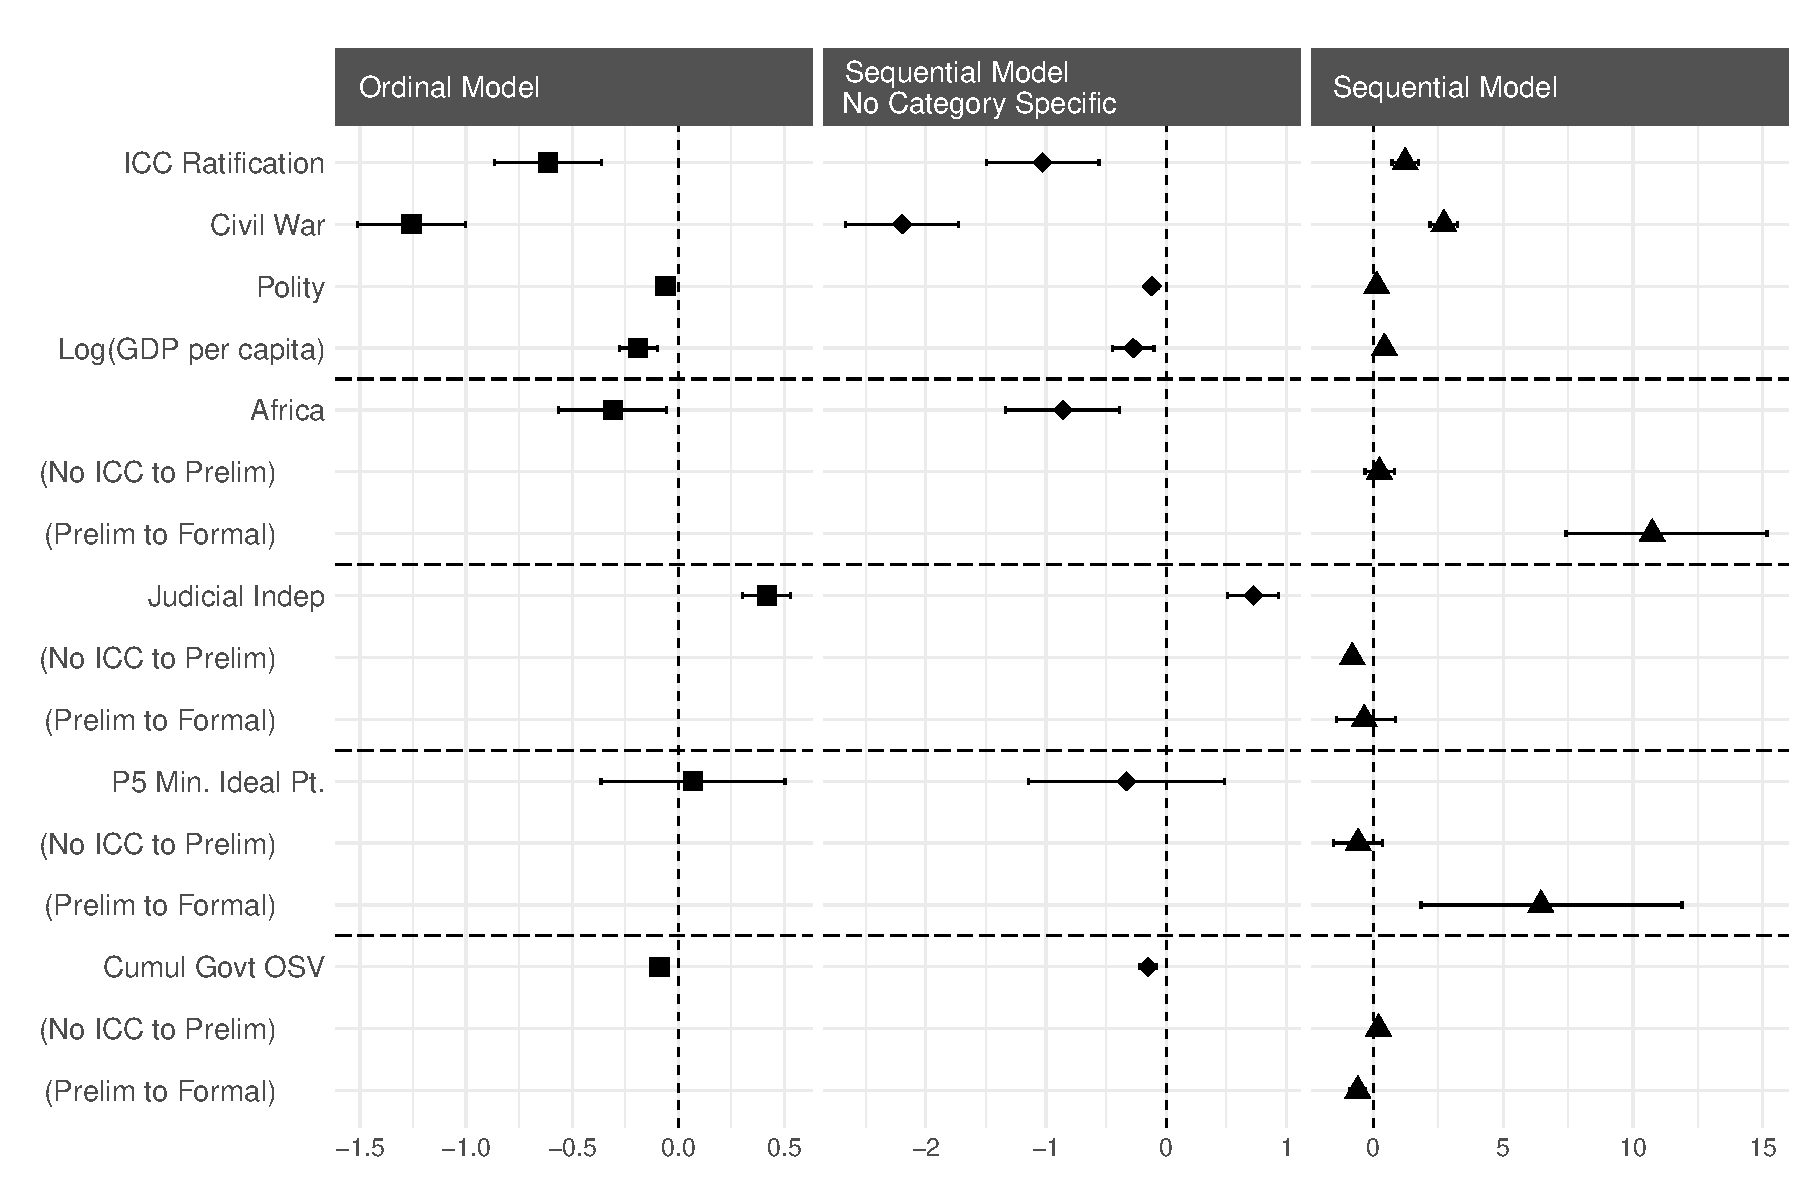
\includegraphics[width=1\textwidth]{modCompare_state.pdf}
    \caption{State model.}
    \label{fig:stateCoefCompare}
\end{figure}

\begin{figure}
    \centering
    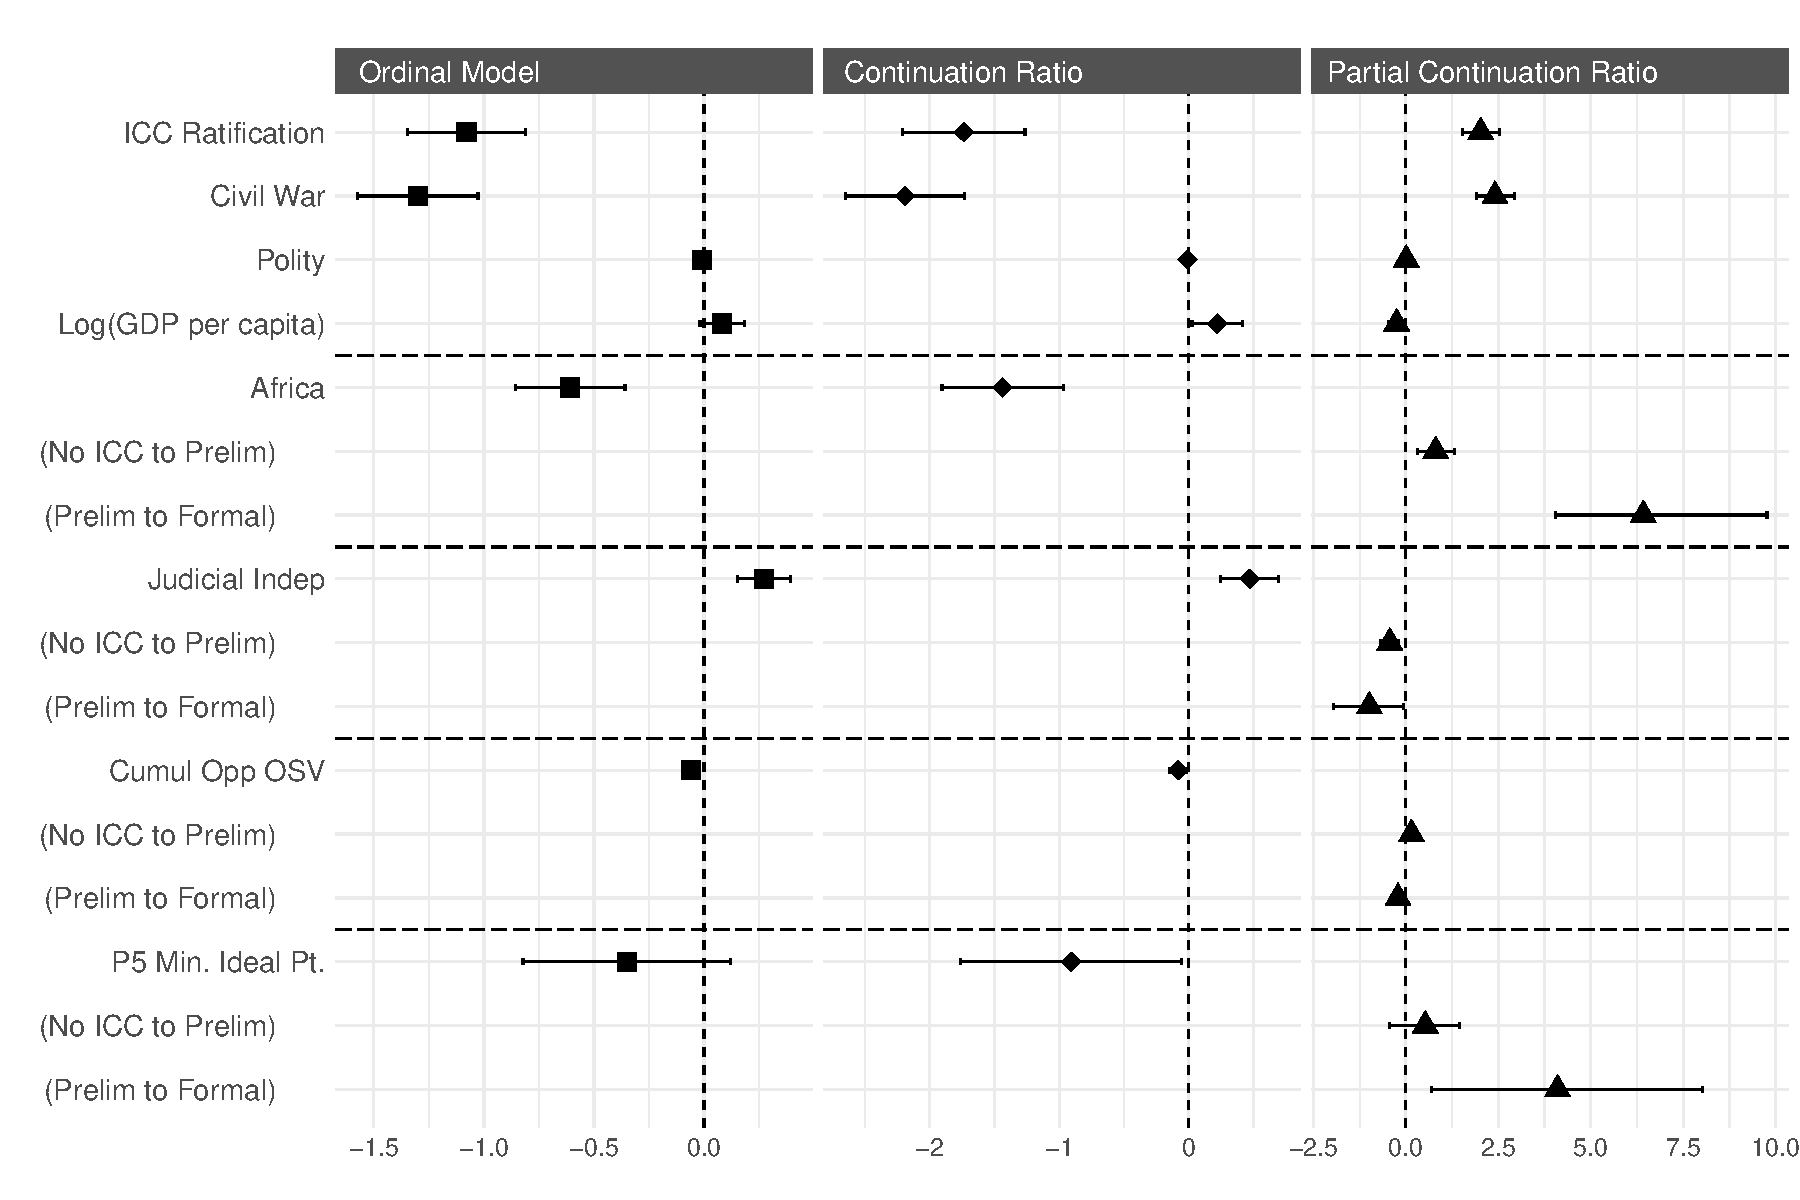
\includegraphics[width=1\textwidth]{modCompare_opp.pdf}
    \caption{Opposition model.}
    \label{fig:oppCoefCompare}
\end{figure}

For ordinal variables the choice of a fit statistic is not as obvious. We use Somer's $D$, a rank correlation coefficient  \citep{Somers1962}, as our discrepancy statistic for the ordinal logit models. Somer's $D$ is closely related to Goodman and Kruskal's $\gamma$ and Kendall's $\tau$, differing only in the denominator.\footnote{Somer's $D$ is similar to the commonly used $\tau_b$, which is equal to $\frac{P - Q}{(P+Q+X_0)(P+Q+Y_0)}$, where $Y_0$ is the number of ties in $Y$, and $\gamma$, which is equal to $\frac{P - Q}{P + Q}$.} Somer's $D$ makes a distinction between the independent and dependent variable in a bivariate distribution, correcting for ties within the independent variable. With $Y$ being treated as the independent variable it is denoted $D_{xy}$.

Specifically:
$$D_{xy} = \frac{P - Q}{P + Q + X_0}$$

\noindent where $P$ is the number of concordant pairs, $Q$ is the number discordant pairs, and $X_0$ is the number of ties in $X$. This is simply a measure of association for ordinal variables, so our approach is essentially to calculate the correlation between predicted and observed values. Like all correlation coefficients, the $D$ statistic lies in the interval $[-1, 1]$, with values closer to $1$ indicating more rank agreement and values closer to $1$ indicated less rank agreement, so values closer to 0 indicate more prediction error.

\begin{figure}
    \centering
    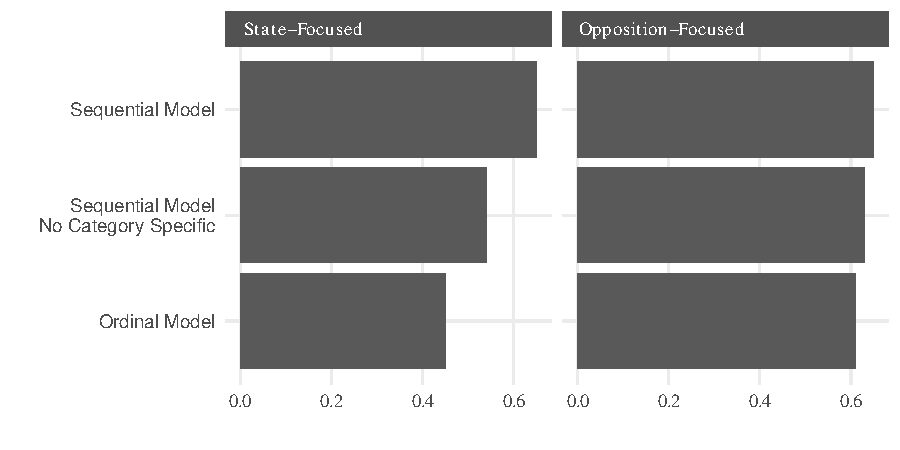
\includegraphics[width=1\textwidth]{somerViz.pdf}
    \caption{Performance comparison.}
    \label{fig:somersD}
\end{figure}
